\documentclass{article}
\usepackage{blindtext}
\usepackage[T1]{fontenc}
\usepackage[utf8]{inputenc}
\usepackage[margin=1in]{geometry}
\usepackage{url}
\usepackage{hyperref}
\usepackage{amsfonts}
\usepackage{graphicx}
\usepackage{caption}
\usepackage{subcaption}
\usepackage{setspace}


\begin{document}

\onehalfspacing
% \doublespacing

\begin{center}

%\LARGE{\textbf{Research Proposal}} \\
%\vspace{1em}
\Large{15-418 Final Project Report} \\
\vspace{1em}
\normalsize\textbf{Manish Nagireddy (mnagired) and Ziad Khattab (zkhattab)} \\
\vspace{1em}

\end{center}

\section*{Title}

An Exploration of Parallelism in Neural Networks

\section{Summary}

For our 15-418 final project, we looked into potential axes of parallelism that exist within neural networks. We implemented image classifying neural networks in \texttt{Python} (via \texttt{PyTorch} and \texttt{mpi4py}, a message passing package for Python) as well as also via \texttt{OpenMP} in \texttt{C++} and measured their performance (e.g. test set accuracy and training time). We found that data parallelism through varying batch size is far more robust (as well as more effective) than attempting to map neural network training to either a shared memory or message passing setting.

\section{Background}

In recent years, we have seen the rapid increase of neural networks within the landscape of artificial intelligence, and more broadly within algorithmic decision making. However, because of the large size of these models (as defined by the number of parameters) as well as the large size of the data used to train them, performance of these so-called deep learning paradigms might be suboptimal without specific attention to parallelism.

Broadly, from the perspective of a neural network, there are two dimensions to parallelize: the data and the model.

\paragraph{Data Parallelism} given $X$ machines/cores, we split the data into $X$ partitions and use the \textit{same} model to train each partition of the data on a different device in parallel. Then, we combine the resultant model weights from each partition. Note that this is \textit{model agnostic} because it relies only on the data and not on the underlying model architecture.

\paragraph{Model Parallelism} splitting the model into various partitions and assigning them to different machines. Note that there are dependencies which are specific to specific model architectures, and so model parallelism is not really ``parallel" because we are actually just assigning consecutive layers of a model to different devices. Some have referred to this as \textit{model serialization}\footnote{\href{https://leimao.github.io/blog/Data-Parallelism-vs-Model-Paralelism/}{Data Parallelism VS Model Parallelism in Distributed Deep Learning Training - Lei Mao's Log Book}}. Model parallelism is commonly used when the model is too large to fit on a single device. \\

\noindent Refer to the figure\footnote{\href{https://xiandong79.github.io/Intro-Distributed-Deep-Learning}{Link to Figure Citation}} below for an illustration of data parallelism and model parallelism.

\begin{figure}[h]
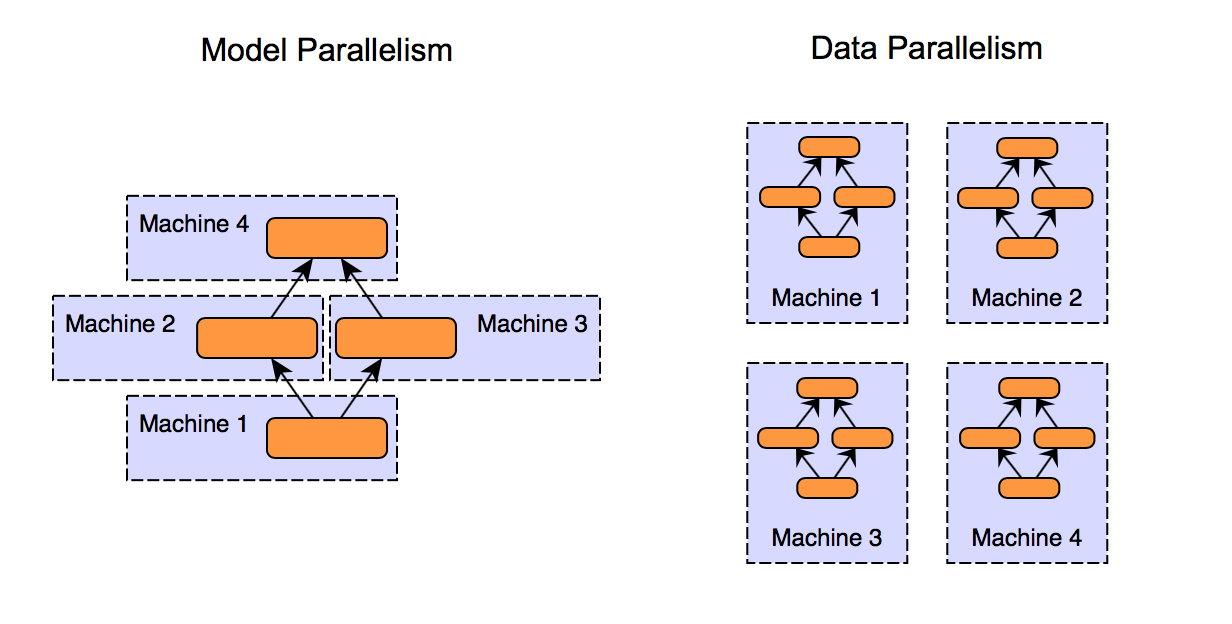
\includegraphics[scale = 0.5]{background}
\centering
\end{figure}

\subsection{Breaking it Down}

The main challenge stems from the fact that there exist a lot of dependencies when working with a neural network. At the lowest, implementation-detail level, we know that different architectures have different structures and therefore different dependencies between layers (e.g. between input and hidden layers). But we also know that the choice of hyperparameters (e.g. learning rate) and optimizers (e.g. Stochastic Gradient Descent or SGD, Adam, AdaGrad, etc.) heavily influence model convergence time as well as model performance. In addition, we have that the choice of dataset is also significant (and related) to the class of models we use. Finally, we are limited by the choice of compute power, in the sense that we can only measure performance on machines with fixed number of CPU cores as well as fixed numbers of GPUs.

Given that we want to focus on parallelism, we did \textit{not} want to get caught up in trying out different models on different datasets with different parameters. Thus, we fixed our dataset to be the widely well-known benchmark MNIST\footnote{\href{http://yann.lecun.com/exdb/mnist/}{Link to MNIST Data}} dataset. This also limited us to the problem of image classification, which further restricted the class of neural networks that we looked at (e.g. now we focused on simple feed forward networks and basic convolutional neural networks or CNNs). From background research, this dataset is known to be relatively cheap to train and still have nontrivial results without excessive preprocessing of the input data. Finally, we decided to hold several commonly used hyperparameters constant. For example, our choice of loss criterion was cross entropy loss, our choice of optimizer was stochastic gradient descent (SGD). So, we fixed these values and varied other hyperparameters, such as the learning rate of the optimizer, the number of training iterations (i.e. epochs), and the batch size. Of course, we also varied the number of processors (in the context of message passing) as well as the number of threads (for shared memory).

Then, we were able to focus the ``unknown" aspects of our project to be the axes of parallelism and their corresponding performance or speedups. Specifically, once we had a baseline working model in \texttt{PyTorch}, we were able to incorporate message passing and then we were even able to implement a shared memory version in \texttt{C++} via \texttt{OpenMP}.

Given that the majority of this class is focused on parallelism, we want to incorporate one of the main kinds of parallel settings that we have talked about. Specifically, in the context of neural network training, it makes sense to use message passing where we can distribute the training across processors. We will have each processor train a copy of the network and then send back the updated weights to a master process. Then, we average the weights together and continue with validating our model via evaluation on a held-out testing set of images. \\

\noindent At a high level, our learning objectives were to
\begin{enumerate}
  \item Think about the inherent dependencies within a deep learning pipeline when attempting to implement a neural network via message passing (and possibly also via shared memory)
  \item Comment on the effectiveness (i.e. speedup and overall performance) of data parallelism in the example of a reasonably complex data and model setting
\end{enumerate}

\subsection{Changes Along the Way}

\paragraph{Dropping \texttt{C++} (for now)}

We note that our project changed immediately following our proposal feedback. For the time being, we decided to drop the \texttt{C++} and \texttt{OpenMP} implementation entirely due to potential time constraints. Then, we changed our project to have the core of the parallelism implementation have to do with \texttt{mpi4py} since we were able to more easily justify how message passing can be leveraged in neural network training (see above).

\paragraph{Dropping Model Parallelism in favor of Message Passing + More Complex Architectures}

Then, after a week or so, when we finished the \texttt{MPI} based implementations of a feedforward multi-layer perceptron (MLP) as well as a basic convolutional neural network (CNN), we decided that the implementation of model parallelism is not rigorous enough to justify the time spent attempting to gather the resources to test model parallel workflows. Specifically, given \texttt{PyTorch} and its capabilities, the way to implement model parallelism would be to send different layers of a network architecture to different machines (e.g. different GPUs). Then, in order to test this model, we would have to secure multi-GPU machines, which would take more work than the actual implementation of model parallelism itself.

Therefore, to account for this change, we decided to translate our message-passing based parallelism to a more sophisticated neural network architecture, such as \texttt{ResNet}. More concretely, given that the internal architecture of \texttt{ResNet} is inherently more complicated than a 2-layer CNN (which we have already implemented), we anticipated that attempting to integrate message passing (again via \texttt{mpi4py}) will be more complicated with respect to implementation. Additionally, we would be able to compare the effectiveness of message passing effects on baseline models against more complicated architectures. This added dimension of comparision, as well as the increase in complexity of implementation, allowed us to justify the change in plans. As we describe later in the results section, the addition of message passing to a more sophisticated model architecture yielded some surprising performance metrics.

\paragraph{The Return of \texttt{C++} }

Finally, with about a week to go before the project deadline, we decided to go for our "Hope to Achieve" goals where we wanted to experiment with moving to \texttt{C++} and potentially also incorporating a shared memory setting via \texttt{OpenMP}. Although it was certainly nontrivial to mesh our idea of data parallelism within the shared memory paradigm, we were able to achieve a successful implementation with decent speedup after thinking carefully about synchronization. We elaborate more on our approach below and on our results further below.

\section*{Approach}

Our approach, in a broad sense, was data-side parallelization of the neural network training process. We did this by partitioning the data across threads, so that different processors are training the neural network architecture from their own randomized starting points, then either using a reductive combination process across all the weights trained by each processor to unify them (in the message passing case) or using synchronization to update a shared copy of these weights (shared memory).

In both the message passing and shared memory settings, we aimed to map a portion of the training data in a given epoch to a processor core. This was the primary basis of parallelism in our codebase.

Given that we want to explore the differences in axes of parallelism, we tried to not spend too much time implementing sequential neural networks from scratch. For \texttt{Python}, we will rely upon the \texttt{PyTorch} documentation for commonly used neural networks (e.g. standard CNN or basic \texttt{ResNet}). The main coding portion (in \texttt{Python + mpi4py}) will come from incorporating message passing into a \texttt{PyTorch} based model.

\paragraph{Message Passing}

The \texttt{Python} portion of the code included two networks, a simple Convolutional Neural Network (CNN), and a more complicated CNN with underlying \texttt{ResNet}\footnote{\href{https://pytorch.org/hub/pytorch_vision_resnet/}{Link to PyTorch ResNet}} architecture. In these two cases, the parallelization was done in a nearly identical way: we had a master process that would send a copy to each worker and then use \texttt{MPI} to broadcast a message to the workers to begin training. The workers would run their training loops and send their state dictionaries (which contained the updated weight parameters for each corresponding model) back to the master to be combined with one another for the next epoch (i.e. next iteration of the training loop). Since we were concerned with parallelization rather than machine learning, we first coded up a simple neural network without any message passing in \texttt{PyTorch} (referring to their documentation for both CNN's and \texttt{ResNet}) to serve as a sequential basis for our code.

There were slight changes to the serial algorithm, in that we had to employ a reductive combination on the weights after the distributed training. This is slightly different from a purely sequential neural network where each input updates the weights cumulatively. We observed some tradeoffs because of this, which we discuss below in our results section.

Optimization mainly occurred in two passes: the initial parallelization, and then the later efforts to make it more efficient. Initially, we used a roundtrip system in \texttt{MPI} to pass the weights on, hoping to emulate the structure of a sequential neural network. Then, the main optimization involved using broadcasting to make the master-worker architecture more efficient, instead of using the aforementioned roundtrip system.

\paragraph{Shared Memory}

The \texttt{C++} portion only used a simple feedforward multi-layer perceptron, but instead used \texttt{OpenMP} to parallelize the training process. The principle was similar, except that there was no need to separate things into master and worker processes because \texttt{OpenMP} allows for automatic work distribution across threads. We note that from the \texttt{C++} standpoint, there exists an abundance of starter code for basic neural networks (e.g. \href{https://github.com/Whiax/NeuralNetworkCpp/tree/master/src/neural}{[1]}, \href{https://github.com/huangzehao/SimpleNeuralNetwork/blob/master/src/neural-net.cpp}{[2]}, \href{https://github.com/arnobastenhof/mnist/tree/master/src}{[3]}). So, once we had a working sequential neural network, we spent an overwhelming majority of the time trying to adapt this implementation into a shared memory setting.

In \texttt{OpenMP}, we used a similar structure to what we have now, but had very conservative lock-based synchronization to ensure correctness, since we did not have the message-passing abstraction to keep things clean and were instead updating weights in shared memory.

We made optimizations by limiting synchronization and minimizing critical sections as much as possible (so much so that in fact we were able to reduce them to two lines in the training loop). Another major breakthrough for us was to make the ``memory windows" used for intermediate weight calculations \textit{private} to the threads instead of shared, and this allowed us to reduce synchronization significantly. This did seem to come with overall memory tradeoffs which we will discuss later in our results section.

\section{Results}

At a high level, we were successful in achieving our main goal - to have a working implementation of our models in a message passing setting so that we will be able to comment on performance and speedup. Additionally, we were even able to achieve one of our extra credit options where we were able to implement a simple feedforward convolutional neural network in \texttt{C++} and combine this with our knowledge of shared memory via \texttt{OpenMP}.

\subsection{Related Work}

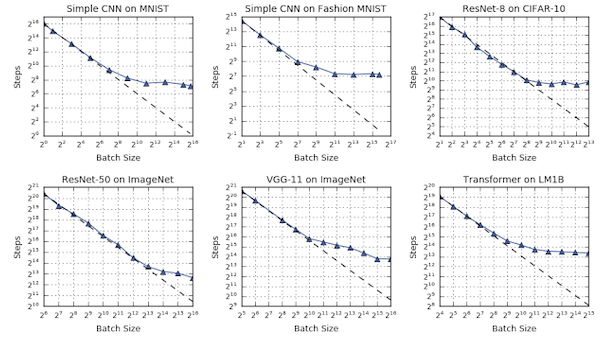
\includegraphics[scale = 0.75]{google}

Before we get into our specific results, we'd like to note that there is a very interesting article from folks at Google Research\footnote{\href{https://ai.googleblog.com/2019/03/measuring-limits-of-data-parallel.html}{Measuring the Limits of Data Parallel Training for Neural Networks}} which describes the various scaling patterns that they observed during data parallelism. Note that their measurement of data parallelism is directly related to the batch size, which is the number of training data examples utilized in one iteration of training the model. Specifically, they discovered three distinct but related so-called ``scaling-regimes":
\begin{enumerate}
  \item Perfect Scaling: doubling batch size halves number of training steps to reach some target error
  \item Diminishing Returns: fewer decreases to training time with increasing batch size
  \item Maximal Data Parallelism: further increasing batch size beyond this point doesn’t reduce training time
\end{enumerate}

\noindent See the figure above for a visual depication of these regimes. Specifically, the Google researchers found a universal relationship between batch size and training speed with three distinct regimes: perfect scaling (following the dashed line), diminishing returns (diverging from the dashed line), and maximal data parallelism (where the trend plateaus). The transition points between the regimes vary dramatically between different workloads\footnote{\href{https://ai.googleblog.com/2019/03/measuring-limits-of-data-parallel.html}{Link to Original Article: ``Measuring the Limits of Data Parallel Training for Neural Networks"}}. We attempted to see if this pattern could also be observed with our model and comment on any differences below in our results section. Note that the Google researchers use training steps, whereas we utilize training time (given by the number of seconds needed to fully complete one epoch of training). This is a simplification for clarity, but one which does not impact correctness since training time and number of training steps are very closely related.

\subsection{Summary of Findings}

\noindent For a quick summary of our findings, we were able to observe similar results as the Google researchers, even in the context of message passing. Specifically, we observed that increasing the batch size resulted in decreasing the training time, but not in a linear fashion. We did, in fact, observe the ``diminishing returns" noted above. Furthermore, we found that increasing the batch size also resulted in lower testing accuracy, which means that our model became poorer at generalizing. Somewhat surprisingly, this pattern was consistent throughout all processor counts (1, 4, 16, 64, and 128).

Then, for our shared memory model, instead of modifying batch size, we decided to hold batch size constant (at 1, so the model processed training images one at a time) and decided instead to modify the learning rate of the optimizer. We thought to do this to see if changing the workload (as the Google folks pointed out) results in different speedups and performance. Again, somewhat surprisingly, we observed near perfect speedup when going from 1 thread to 4 threads but then saw degradation and eventual deterioration for higher thread counts (e.g. 64 and 128).

\subsection{Visualizations and Further Analysis}

\subsubsection{Varying Batch Size}

Our primary set of experiments involved attempting to see if the Google Research ``scaling regimes" (i.e. perfect scaling, diminishing returns, and maximal data parallelism) held true even after we incorporated message passing.

\begin{figure}[!h]
    \centering
    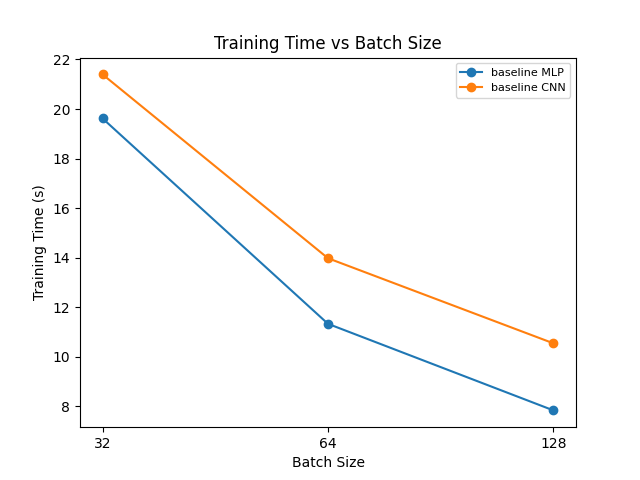
\includegraphics[scale=0.5]{base_time_bs}
    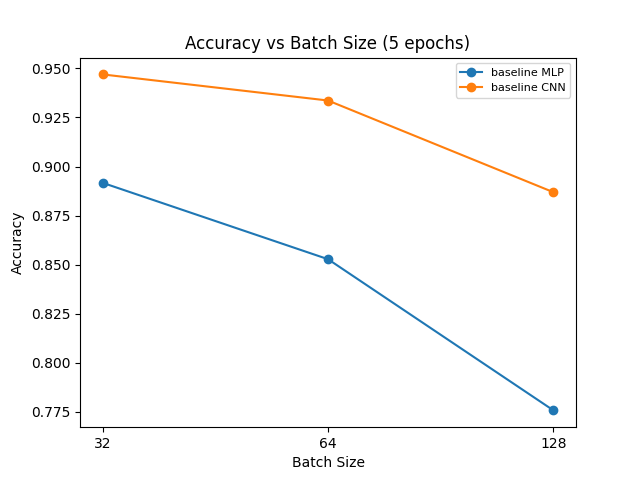
\includegraphics[scale=0.5]{base_acc_bs}
    \caption{Plots of training time for 1 epoch and accuracy (after 5 epochs of training) with learning rate of 0.01 for both baseline MLP and baseline CNN models. Note, there is \textit{no} message passing in either of these models, as they are our reference points.}
    \label{fig:base_bs}
\end{figure}

\paragraph{Baseline Models}

First, we implemented two sequential models which served as a baseline for comparisons. Our most basic model is a simple 2-layer feed-forward multi-layer perceptron (referred to as our baseline MLP in the figures). Then, our second baseline model is a convolutional neural network (CNN) with 2 convolutional layers (referred to as our baseline CNN in the figures).

Now, look to Figure \ref{fig:base_bs} for the plots of training time and accuracy across varying batch sizes. Specifically, we point to the fact as we double the batch size from 32 to 64, we see \textit{almost halving} the training time. This corresponds to the ``perfect" scaling regime from the Google Research folks. However, going from batch size of 64 to 128 results in a less than half reduction in training time. So, this corresponds to the ``diminishing returns" regime. However, note that there is still a decrease in training time, so we have not yet reached the point of ``maximal data parallelism" where increasing batch size no longer decreases the training time. Then, in the accuracy plots, we see that increasing the batch size decreases the accuracy at an almost (but not quite) linear rate.

Note that this phenomenon is studied quite in depth in the literature, where we found that ``Practitioners often want to use a larger batch size to train their model as it allows computational speedups from the parallelism [of GPUs]. However, it is well known that too large of a batch size will lead to \textit{poor generalization}"\footnote{\href{https://medium.com/mini-distill/effect-of-batch-size-on-training-dynamics-21c14f7a716e}{Link to Article: ``Effect of batch size on training dynamics"}}.

\paragraph{Message Passing Model}

\begin{figure}[!h]
    \centering
    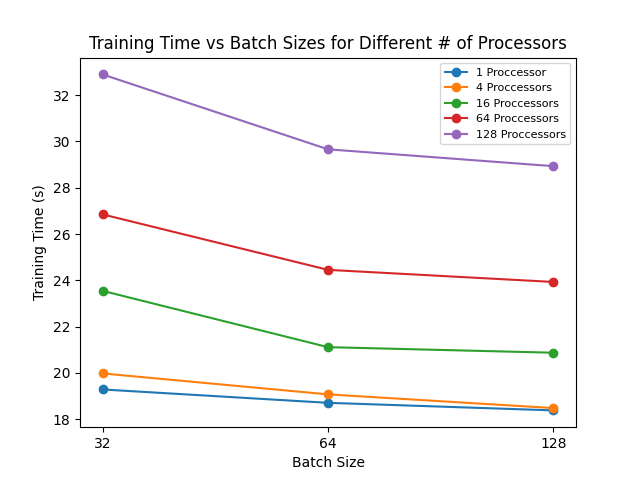
\includegraphics[scale=0.5]{cnn_mpi_bs_time}
    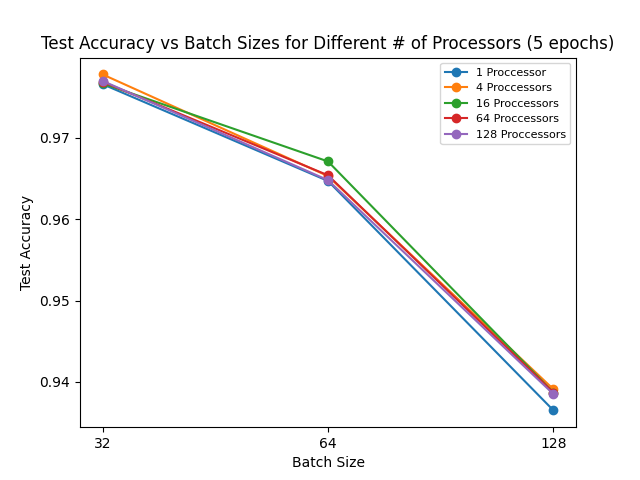
\includegraphics[scale=0.5]{cnn_mpi_bs_acc}
    \caption{Plots of training time and speedup for 1 epoch and accuracy (after 5 epochs of training) with learning rate of 0.01 for CNN model \textit{with message passing}.}
    \label{fig:cnn_bs}
\end{figure}

We modified our baseline CNN model to also integrate message passing (via the \texttt{mpi4py} package). As described above in our approach section, this required that different processors are training the neural network architecture from their own randomized starting points, and then the master process utilizes a reductive combination process across all the weights trained by each worker processor to unify them into one updated weight matrix.

Now, look to Figure \ref{fig:cnn_bs} for the plots of training time, speedup, and accuracy across varying batch sizes. Specifically, we see that the training time follows a similar trend as for the baseline models where going from batch size of 32 to 64 results in a larger decrease than going from 64 to 128. However, one thing to note is that we no longer experience any perfect scaling due to the inclusion of message passing. We are immediately thrust into the ``diminishing returns" regime. We believe this is due to the fact that the size of the messages being passed is too large and therefore dominates the computation time. As stated above, our message passing neural network works by sending copies of the weights (via the model's internal state dictionary) to all of the worker processes. This is an extremely large (and dense) matrix, which results in a lot of communication. We see this is evident by the physical training times needed by the message passing model. Observe that even for the simplest message passing model (which only uses 1 worker process), the need to send a single message results in over 18 seconds to train 1 epoch with a batch size of 64 (visually, this is the second blue dot on the left plot in Figure \ref{fig:cnn_bs}). For reference, the baseline cnn model was able to train in almost 5 fewer seconds (given by the second blue dot on the left plot in Figure \ref{fig:base_bs}). So, what we observe is that the overhead of message passing is large enough to diminish the reduction in time after increasing batch size, but not enough so as to completely eradicate the effect of doubling batch size.

What we found more surprising was that this pattern, of smaller but still visible reductions in training time due to batch size increases, was apparent across all processor counts. This showed us that our message passing implementation was decent enough to allow the batch size factor to still appear, despite the number of message needing to be sent.

As far as accuracy is concerned, we found similar results as to the baseline models, where increasing batch size resulted in lower testing accuracy. Again, this is largely due to the same factors as previously stated above.

\subsubsection{Varying Learning Rate}

\begin{figure}[!h]
    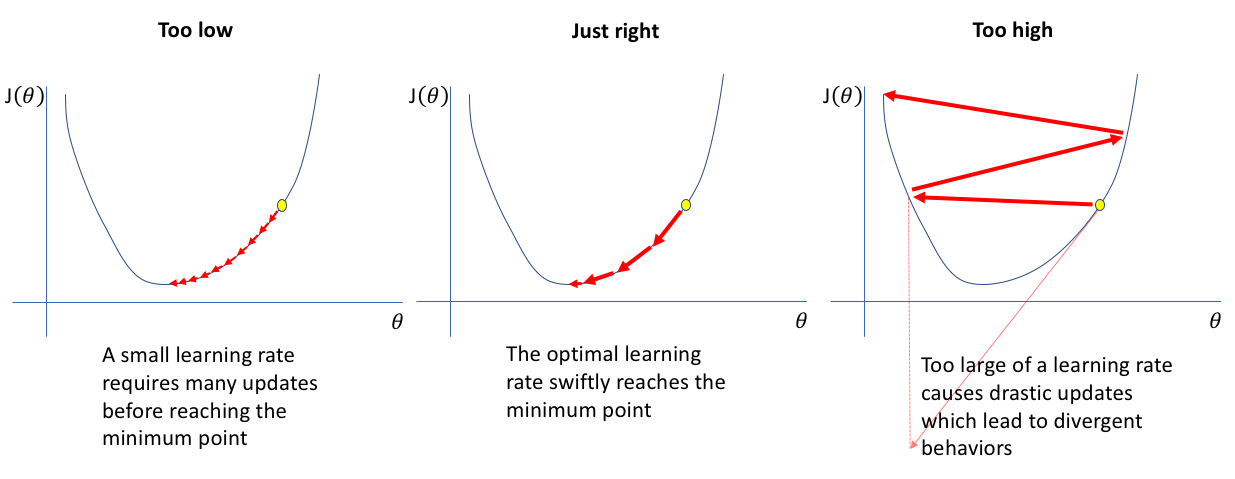
\includegraphics[scale = 0.35]{lr}
    \centering
    \caption{Explanation of learning rate size on neural network convergence.}
    \label{fig:lr}
\end{figure}

As an additional axis of comparison, we decided to hold batch size and number of training epochs constant (512 and 5 respectively) and vary the learning rate of the stochastic gradient descent (SGD) optimizer. We varied the learning rate to be in the set $\{0.0001, 0.001, 0.01, 0.1, 1, 10\}$. Additionally, we wanted to see whether varying the number of processors (for message passing) or the number of threads (for shared memory) resulted in different accuracies or training times due to the size of the learning rate. For reference on what learning rate means in the context of the deep learning pipeline, refer to Figure \ref{fig:lr}.

\begin{figure}[!h]
    \centering
    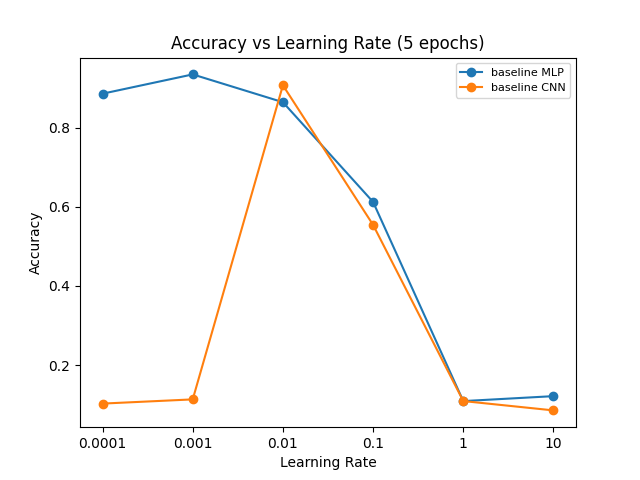
\includegraphics[scale=0.5]{base_acc}
    \caption{Plot of accuracy (after 5 epochs of training) with varying learning rates for both baseline MLP and baseline CNN models. Note, there is \textit{no} message passing in either of these models, as they are our reference points.}
    \label{fig:base_lr}
\end{figure}

\paragraph{Baseline Models}

Since the baseline models don't have any explicit parallelization, it doesn't make sense to collect their training times for varying learning rates. Instead, we look at their testing accuracies (Figure \ref{fig:base_lr}) and find that a learning rate of 0.01 appears to be the most optimal, because it resulted in the best training accuracy, which means the model with the highest predictive power.

\paragraph{Message Passing Models}

\begin{figure}[!h]
    \centering
    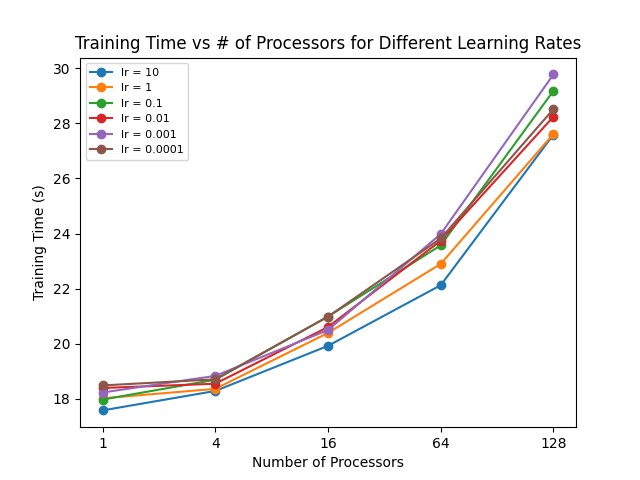
\includegraphics[scale=0.5]{cnn_mpi_lr_time}
    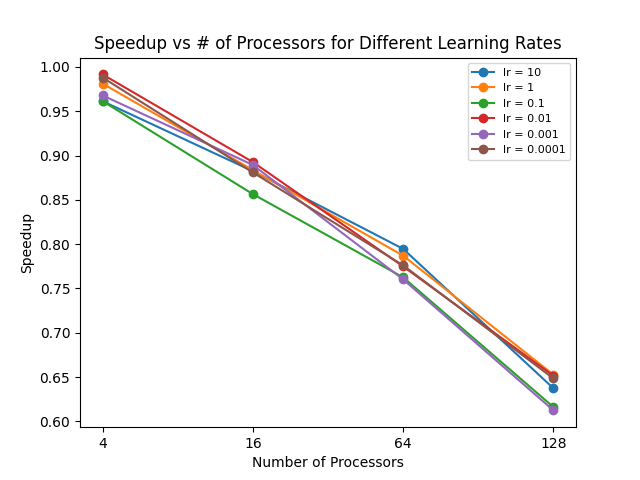
\includegraphics[scale=0.5]{cnn_mpi_lr_speed}
    \caption{Plots of training time and speedup for 1 epoch with varying learning rates for CNN model \textit{with message passing}.}
    \label{fig:cnn_lr}
\end{figure}

Now, we first display the results of experiments on the CNN model with message passing in Figure \ref{fig:cnn_lr}. From these plots, we can observe that the training time increases almost exponentially as we increase the number of processors. As stated before, this is largely due to the size of the messages that need to be sent.

Again, somewhat surprisingly, we see that the training time increases in similar fashions for all learning rates. What this means is that even though an extremely suboptimal learning rate might be bad for convergence, the time it takes to train the model is not dependent upon the learning rate, across differing numbers of processors.

\begin{figure}[!h]
    \centering
    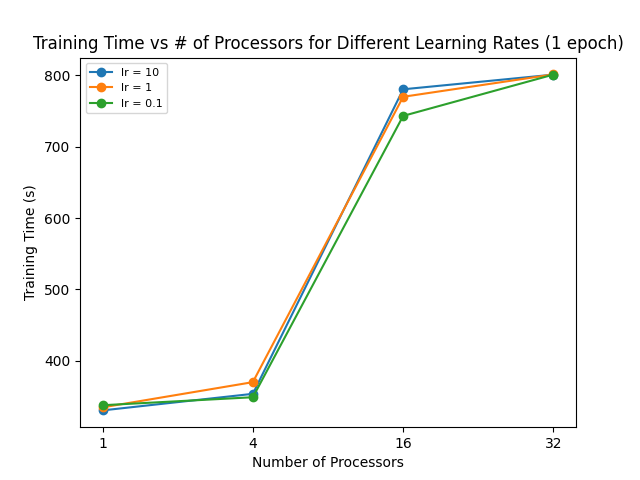
\includegraphics[scale=0.5]{res_lr_time}
    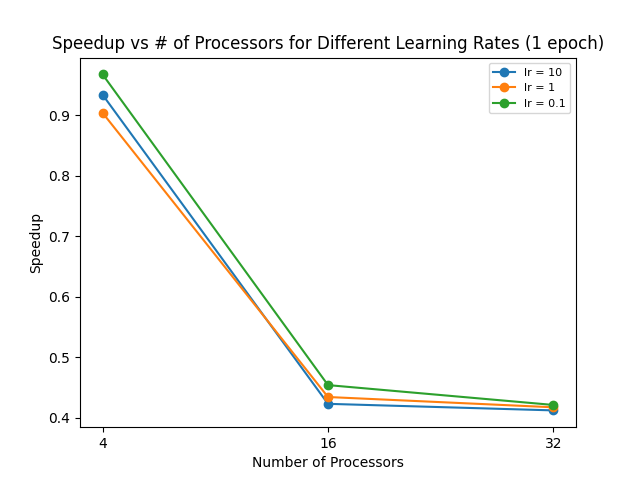
\includegraphics[scale=0.5]{res_lr_speed}
    \caption{Plots of training time and speedup for 1 epoch with varying learning rates for \texttt{ResNet} model \textit{with message passing}.}
    \label{fig:res_lr}
\end{figure}

\begin{figure}[!h]
    \centering
    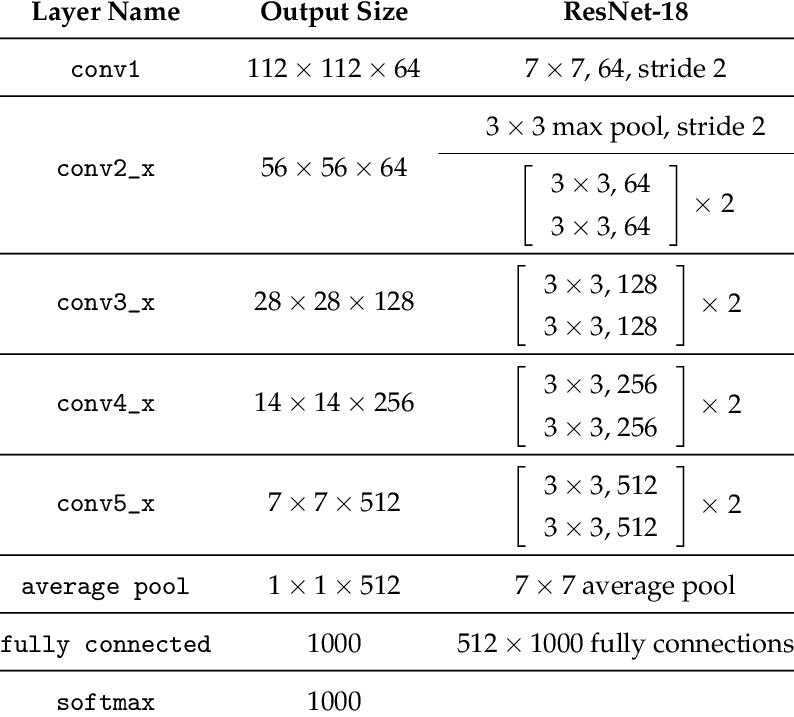
\includegraphics[scale=0.25]{res18}
    \caption{\texttt{ResNet18} model architecture}
    \label{fig:res18}
\end{figure}

Next, we first display the results of experiments on the more complicated \texttt{ResNet} model with message passing in Figure \ref{fig:res_lr}. From these plots, we can observe similar patterns to the simpler CNN from above. However, paying close attention to the physical training time, we see that it takes over 5 \textit{minutes} to train a single epoch of the \texttt{ResNet} model with message passing. This is due to the fact that the \texttt{ResNet} architecture is significantly more complicated, with many more convolutional and fully connected layers, than our original CNN model. Refer to Figure \ref{fig:res18} for a tabular view of the model architecture\footnote{\href{https://www.researchgate.net/figure/ResNet-18-Architecture_tbl1_322476121}{Link to Image}}. Hence, as can be expected, we observe much higher training times due to the fact that the updated weights of the models (which are the messages that are being sent) are significantly larger in size. Additionally, there is also the overhead present of training a larger and deeper neural network which adds extra computation time.

\begin{figure}[!h]
    \centering
    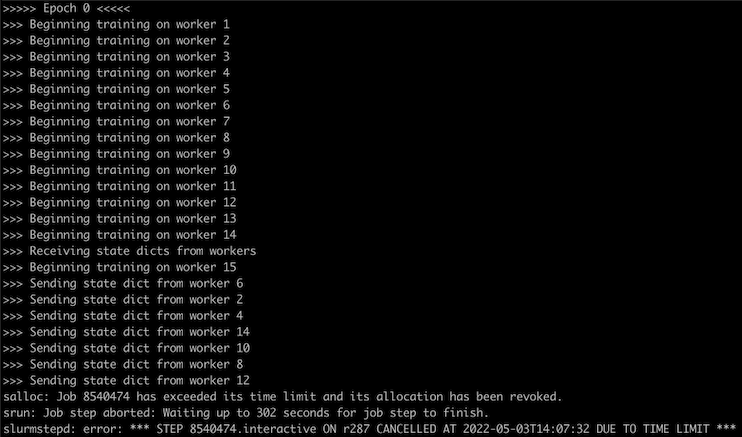
\includegraphics[scale=0.35]{kill_res}
    \caption{An example of PSC killing the job of training our \texttt{ResNet} model with MPI}
    \label{fig:kill_res}
\end{figure}

As you may observe, we do not provide any metrics beyond 32 processors, which is due to the fact that the PSC machines would automatically kill our jobs given the magnitude of time needed to complete the training of the network for higher processor counts. Refer to Figure \ref{fig:kill_res} for an example of the output we obtained.

Nevertheless, we were able to observe that message passing does not work well in terms of training time for more complicated neural network architectures.

\paragraph{Shared Memory}

\begin{figure}[!h]
    \centering
    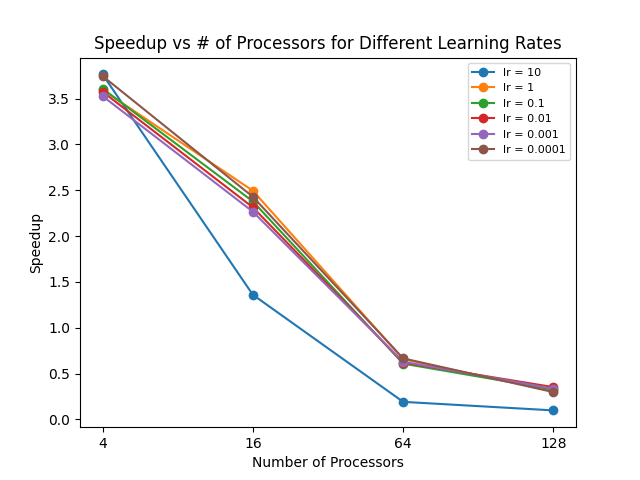
\includegraphics[scale=0.5]{mp_lr_speed}
    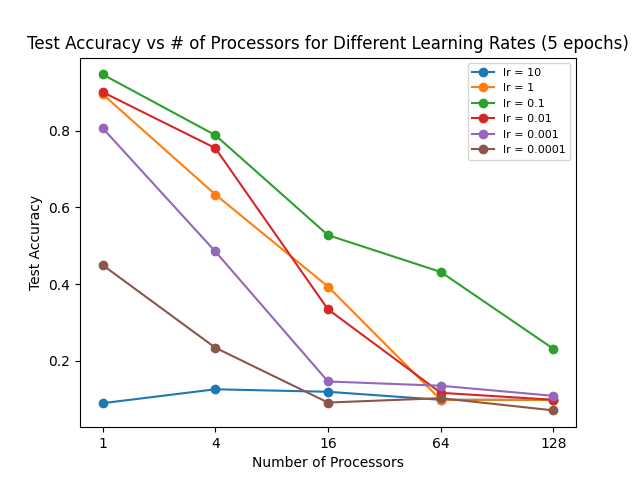
\includegraphics[scale=0.5]{mp_lr_acc}
    \caption{Plots of speedup for 1 epoch as well as accuracy (after 5 epochs) with varying learning rates for \texttt{OpenMP} CNN in \texttt{C++}.}
    \label{fig:mp_lr}
\end{figure}

There were a few patterns observed in the results gathered from the OpenMP experiments on the PSC machines. Refer to Figure \ref{fig:mp_lr} for the plots. Note that we managed to obtain near perfect speedup going from 1 processor to 4 processors, which we delve into below.

The first set of results pertains to the trend of decreasing test accuracy as the processor count increased, across all learning rates (with the possible exception of 10.0, which did very little training at all). Primarily, this is caused by the nature of neural network parallelization across data. Traditionally, a neural network trains on the data sequentially. It starts with randomized weights, then obtains feedback from the first input, then the second, and so on. In the parallel model, $N$ threads are started with their individually randomized weights, and each of the $N$ threads operates on a portion of the data, which is then merged at the end. This improves the speed that the model is able to take in the data, but if Thread 1 handles inputs 1-10, and Thread 2 handles inputs 11-20, they are not able to compound their learning upon one another since they are operating simultaneously. This means that in an equivalent amount of epochs, we expect to see higher parallelism correlate with decreases in test accuracy. The benefit of parallelism is in a long-term trade off, where better utilization of hardware over a correspondingly increased number of epochs is able to achieve the same test accuracy, but in an overall shorter amount of time.

On the other hand, we saw that speedup was decreasing as the number of processors increased, with a U-shaped curve for the amount of time taken to train. Essentially, speedups began at high values moving from 1 to 4 processors, but 1 to 16 saw a smaller speedup, and 1 to 64 and above yielded slowdowns. It is difficult to pin down exactly one reason for this, but there are a number of contributing factors. The first is competition over the resources of the machines being tested, from other processes running on them. This results in poor CPU utilization and wasted thread startup overhead, since additional threads are not being allocated to their own cores. Another reason is a bottleneck in the startup phase of each thread, involving randomization of the initial weights. The random number generator library provided by \texttt{C++} is not designed for multithreaded use. While functional, it relies on global memory access and is not efficient in a parallel context, and likely acts as a bottleneck. It is called tens of times during each thread startup. Furthermore, there are potential random access memory (RAM) concerns due to the fact that each thread allocates its own private large blocks of memory to store the inter-layer weights used in intermediate matrix multiplication calculations. Given that the data being analyzed is images, the sizes can get pretty large, which may lead to severe competition for memory resources on the system. Overall, this would explain why profound speedups are seen at 4 and 16 processors, but strongly diminishing and even negative returns are seen past that point.

An interesting fact is that lower speedup on shared memory based neural networks has been found in prior research literature as well. From the folks at the University of Ulm in Germany, they found that “the reason for the lower speedup of OpenMP-based implementation seems to be the \textit{unavoidable false cache sharing} of data arrays that are frequently modified by several threads.”\footnote{\href{https://citeseerx.ist.psu.edu/viewdoc/download?doi=10.1.1.595.8618&rep=rep1&type=pdf}{Link to Paper: ``A comparison of OpenMP and MPI for neural network simulations on a SunFire 6800"}} In the context of our results, we note that false sharing occurs when data from multiple threads, which was not meant to be shared, gets mapped to the same cache. This can lead to performance where it appears that multiple threads are competing for the same data. Hence, this correlates with what we saw, since the shared weights array is shared between an increasing number of processors. Since they all need to update the summed weights, we observe a situation where each processor is invalidating the caches of the others when it does its own update, leading to poor performance.

\subsection{Closing Thoughts}

Although we were able to verify that the Google Research team's findings regarding batch size and data parallelism exist even after integrating message passing, we found that neural network training is not really amenable at all to message passing. Although we could manage for our smaller and more shallow models, it became too costly to send a copy of the weight matrices for larger and more complex architectures.

Additionally, we note that we only tested on CPUs, whereas we might have benefitted from the internal hardware components of GPUs, which are broadly used for deep learning. The reason we stuck to CPUs was due to the easy of access to higher processor and thread counts via PSC. A possible future direction of our project would be to see if similar results hold when we run our more complex models on a sophisticated GPU.

Nevertheless, we are thankful for the experience of walking through a step-by-step process of integrating both message passing and shared memory ideas into a deep learning pipeline. We hope our results are, at the very least, interesting (as they certainly were to us when we were collecting them!)

\newpage


\section{References}

Each of these links are click-able!

\begin{enumerate}
  \item \href{https://ai.googleblog.com/2019/03/measuring-limits-of-data-parallel.html}{Google Research: Measuring the Limits of Data Parallel Training for Neural Networks}
  \item \href{https://www.pyohio.org/2019/presentations/123}{Distributed Deep Neural Network Training using MPI on Python}
  \item \href{https://leimao.github.io/blog/Data-Parallelism-vs-Model-Paralelism/}{Data Parallelism vs Model Parallelism}
  \item \href{https://web.stanford.edu/~rezab/classes/cme323/S16/projects_reports/hedge_usmani.pdf}{Parallel and Distributed Deep Learning}
  \item \href{https://cse.buffalo.edu/faculty/miller/Courses/CSE633/Ma-Spring-2014-CSE633.pdf}{Parallel Implementation of Deep Learning Using MPI}
  \item \href{https://analyticsindiamag.com/a-guide-to-parallel-and-distributed-deep-learning-for-beginners/}{A Guide to Parallel and Distributed Deep Learning for Beginners}
  \item \href{https://arxiv.org/pdf/1404.5997.pdf}{Variable Batch Size}
  \item \href{https://citeseerx.ist.psu.edu/viewdoc/download?doi=10.1.1.595.8618&rep=rep1&type=pdf}{OpenMP + NN research paper}
  \item \href{https://www.cs.swarthmore.edu/~newhall/papers/pdcn08.pdf}{Parallelizing Neural Network Training for Cluster Systems}
  \item \href{https://www.jeremyjordan.me/nn-learning-rate/}{Learning Rate Overview}
  \item \href{https://towardsdatascience.com/an-overview-of-resnet-and-its-variants-5281e2f56035}{ResNet Architectures}
  \item \href{https://medium.com/mini-distill/effect-of-batch-size-on-training-dynamics-21c14f7a716e}{Batch Size vs. Training Dynamics}
  \item \href{https://pytorch.org/tutorials/intermediate/model_parallel_tutorial.html}{Single-Machine Model Parallel Best Practices - PyTorch}

\end{enumerate}


\section{List of Work}

\begin{itemize}
  \item Manish Nagireddy (mnagired)
  \begin{enumerate}
    \item Initial Project Ideation
    \item Background Research
    \item Implementing baseline models in \texttt{Python}
    \item Adding MPI functionality to CNN model in \texttt{Python}
    \item Adding MPI functionality to \texttt{ResNet} model in \texttt{Python}
    \item Running Experiments on PSC
    \item Final Report: summary, background, approach, and results
  \end{enumerate}
  \item Ziad Khattab (zkhattab)
  \begin{enumerate}
    \item Background Research
    \item Implementing baseline model in \texttt{C++}
    \item Adding MPI functionality to \texttt{OpenMP} model in \texttt{C++}
    \item Running Experiments on PSC
    \item Final Report: Approach and results for \texttt{C++} models
  \end{enumerate}
\end{itemize}

We stress that equal contributions were made by both students!

\end{document}
